
\documentclass[11pt,letterpaper]{article}
% \documentclass[11pt]{report}
% \documentclass{report}
% \documentclass{book}
\usepackage[bookmarks]{hyperref}
\usepackage{amssymb,amsmath}
% \usepackage{fullpage}
\usepackage{tabulary}
\usepackage{tabularx}
\usepackage{float}
% \usepackage[margin=1.00in]{geometry}
\usepackage[margin=0.90in]{geometry}

\usepackage{caption}
\usepackage{booktabs}
\usepackage{pslatex}
\usepackage{apacite}
\usepackage{subcaption}
\usepackage{pgfplots}
\usepackage{wrapfig}
\usepackage[english]{babel}
\usepackage{lmodern}
\usepackage{setspace}
\doublespace
% \usepackage{url}
\usepackage{bigfoot}
\usepackage[export]{adjustbox}
\setlength\intextsep{0pt}

\usepackage{graphicx}

\title{Model and results for identity signaling project}

\author{{Paul E.~Smaldino and Matthew A.~Turner}}

\begin{document}
\maketitle

\section{Introduction}

When we interact with others it is often to mutually benefit from the
exchange. For instance, we shop at a store to buy things we want from one or
a group of people who want to do the hard work of shopkeeping. When we are
dissimilar from those with whom we interact, the benefit can be lessened.
For instance, you might be wearing a shirt with a political slogan and 
the shopkeeper has posted signs boasting their political affiliation. Perhaps
the shopkeeper decides to charge you more, or perhaps you feel a sense of 
resentment for giving money to someone with whom you disagree politically;
maybe the shopkeeper's signage distracted you from making all the purchases 
you needed to make. Shopping is rather inconsequential, but illustrates the issue. 
A much more critical situation is the interaction of political partisans, who
must mutually benefit one another for democracy to work.

In response to the fact that
interpersonal disliking often lowers payoffs from interaction, humans have
developed \emph{covert signaling} strategies so that, e.g.,
customer and shopkeeper can signal their political affiliations so that like-minded
people will know they are similar, but dissimilar others will be unaware
of political or identity signaling at all. Different social settings present
different signaling pressures. Sometimes it is possible to choose who we assort
with for interaction, which means the practice of homophily---selectively
interacting with similar others---is widespread. In that case, there is little
reason to signal covertly because we can preferentially 
interact with similar others, avoiding penalties for interaction with 
dissimilar others. Sometimes the penalties for
disliking one another are very high, which pressures individuals to choose
covert signaling more often in order to not be disliked. While there are
interaction costs for dislike there are benefits for the case where two, which are
also included in the model.

Here we present a model of identity signaling, social interaction,
and social learning to identify mechanisms for the evolution of the covert 
signaling strategy, as opposed to an overt signaling strategy. The precise 
definitions of overt and covert signaling are given in the Model section.
Our results are thus predictions of when covert signaling will or
will not evolve. This depends on a number of model parameters and the 
co-evolution of the \emph{receiving} strategy, which may be either \emph{generous}
or \emph{churlish}. Generous individuals do not dislike
others with whom they have not previously interacted. Churlish individuals 
dislike others with whom they have not previously interacted.

The model predicts that covert signaling evolves when homophily is low (agents
do not efficiently assort) and the costs of disliking are high. The model also 
predicts that covert signaling co-evolves with generous receiving. This is due
to the fact that covert signalers are simply ignored by those with whom
they are different. If most of the individuals are churlish receivers, there is
no benefit to being unknown since most individuals dislike unknown others. 
We also use our model to predict differences in covert signaling prevalence
among minority and majority populations, where the minority and majority all
share the same in-group traits along a number of trait dimensions, but exactly
the opposite traits. If homophily is weak and disliking costs are high, the
minority will tend to become covert signalers. However, if homophily is
sufficiently high it is better for the minority to overtly signal so they can
efficiently identify similar interaction partners. We close by finding the
conditions that promote either signaling or receiving strategies to ``invade'',
i.e.\ become prevalent after starting as just a small fraction of the population.
We find here that sometimes no signaling is better than overt signaling: 
covert signaling can evolve even when the efficiency of covert signaling is
zero, i.e.\ covert signals are not understood by any model individuals (agents).

\section{Model}

The model includes parameters to represent homophily, the penalty for 
individuals who dislike one another, the efficiency of covert signaling, and the
number of traits assumed to be important in social interaction for a model system.
These are summarized in Table~\ref{tab:params} below.

\vspace{1em}
\begin{table}[H]
  \centering
  \begin{tabular}{cp{3.5in}c}
    Symbol & Definition & Values tested (default in bold)  \\
    \toprule 
    $w$      & \emph{Homophily}, the ability of agents to preferentially interact with similar others & $\{0.0, 0.05, 0.10, \ldots, 0.5\}$ \\
    $d$      & \emph{Disliking penalty} imposed when one agent dislikes the other & $\{0.0, 0.05, 0.1,\ldots \mathbf{0.25}, \ldots, 0.5\}$ \\
    $\delta$ & Additional penalty when pair dislike one another & \textbf{0.25} \\
    $E_{cov}$ & \emph{Efficiency of covert signaling} & $\{0.0, 0.05, 0.1,\ldots \mathbf{0.25}, \ldots, 0.5\}$ \\
    $E_{ov}$ & \emph{Efficiency of overt signaling} & \textbf{0.5} \\
    $s$      & \emph{Similarity benefit} received by similar interacting pair & \textbf{??} \\
    $K$      & Number of agent identity traits & $\{\mathbf{3}, 9\}$ \\
    $S$      & Minimum fraction of traits in common for a pair to be considered similar & 
      $\{0.1, 0.2, \ldots, \mathbf{0.5}, \ldots, 1.0\}$\\
    $M$      & Number of traits used to define majority/minority populations & $\{\mathbf{2}, 4\}$\\
  \end{tabular}
  \caption{Global, as opposed to agent-specific, model parameters. 
  Explanatory model parameters are used to answer
  our guiding questions about identity communication strategies. In the final
  column the default value is in bold, if there is one. Homophily never has a
  default value because it is varied in every computational experiment
  condition we test.}
  \label{tab:params}
\end{table}

\subsection{Agents}

Model individuals are \emph{agents} who 
\begin{enumerate}
  \item have static ``in-born'' traits that determine pairwise similarity or dissimilarity
  \item hold attitudes about all other agents in the system
  \item have adopted a signaling and receiving strategy
\end{enumerate}
Signaling strategies
may be either \emph{covert} or \emph{overt}, and receiving strategies may be
either \emph{generous} or \emph{churlish}. Unless otherwise noted, agents are
randomly initialized to be covert or overt with equal probability. The 
proportion of agents with specific signaling or receiving strategies will be
set to different values in the invasion experiments, explained in more detail below.

Agents have $K$ traits, where $K$ is a parameter representing the cultural 
complexity of the system. In the real world, different systems may have 
different cultural complexities. For instance, in United States politics, there
is increasingly little subtlety and increasing partisanship, so $K \approx1 $.
However, if we were trying to understand scholarly positions on some research
question, we may have $K$ be very large, or $K$ could be large if we consider
agents to be, e.g., nations instead of people (as in Axelrod 1997).  

\begin{table}[H]
  \centering
  \begin{tabular}{cp{4.5in}}
    Agent property & Description \\
    \toprule
    $a_{ij}$   & Attitude of agent $i$ towards agent $j$; $a_i$ is the $N$-dimensional 
      attitude vector of agent $i$. \\
    $\tau_{ik}$ & Trait $k$ of agent $i$; $\tau_i$ is the $K$-dimensional trait vector of agent $i$. \\
    Signaling strategy & Either \emph{overt} or \emph{covert}. Overt signaling always
                         results in the communication of the signaler's traits,
                         while covert signalers only reveal their traits to 
                         ``similar'' others; dissimilar others do not receive a covert signal. \\
    Receiving strategy & Either \emph{churlish} or \emph{generous}. Churlish
                         receivers default to dislike other agents from whom they have
                         not received a signal. Generous receivers default to
                         a neutral attitude towards others from whom they have
                         not received a signal.
  \end{tabular}
  \caption{Agent attributes.}
  \label{tab:agentAttributes}
\end{table}


\subsubsection{Determining inter-agent similarity}

Each trait $j$ of agent $i$ takes a value $\tau_{ik} \in \{-1, 1\}$. $-1$ and 1
are used only to emphasize that there are two opposing traits.
Attitudes are $a_{ij} \in \{-1, 0, 1\}$ with meanings of 
disliking, neutral, or liking. Attitudes are set at the signaling and receiving
rounds, explained in more detail below. Briefly, if agent $i$ recieves a
trait signal from agent $j$, $a_{ij}$ will be 1 if the two agents have
similar traits, and $-1$ if $i$ and $j$ are sufficiently different. Similarity
is $s_{ij} = 1 - d(\tau_i, \tau_j)$ where $d(\tau_i, \tau_j)$ is the
Hamming distance between trait vectors. The Hamming distance is the fraction
of vector elements that are different. So, if $\tau_i = (1,~-1,~1)$ and
$\tau_j = (1,~-1,~-1)$, then $d(\tau_i, \tau_j) = 1/3$ and $s_{ij}=2/3$.
Two agents are ``similar'' if their similarity $s_{ij} \geq S$, where
$S$ is the similarity threshold parameter. Otherwise they are considered
dissimilar. 

If two agents are similar, this enables agents to like one another. On the
other hand, dissimilar agents may come to dislike one another if they signal
their traits to one another. As explained further in the following section on
model dynamics, inter-agent attitudes determine the probability agents will
interact; the payoff received when a particular dyad interacts; and the
probability that one agent chooses another as a teacher.

\subsection{Dynamics}

Each model iteration consist of three stages. First, agents signal their identities
to some fraction of all other agents. It is at this step that agent attitudes
$a_{ij}$ are set. Whether or not an agent receives a signal depends on the
efficiency of overt and covert signaling, $E_{ov}$ and $E_{cov}$, respectively.
\emph{Efficiency} is the proportion of agents in the population that receive
a given agent's signal depending on whether the agent is an overt or covert
signaler.  Signals are sent and received once every model iteration. 
If agent $i$ does receive a signal that agent updates its attitudes about
signaler $j$, then $i$ updates its attitudes about $j$ ($a_{ij}$), according to
the process outlined above.

Then agents then
interact at most $N_I$ times with other agents. In each of the possible 
$N_I$ interactions, agents first match with one agent selected randomly from
the population. The probability these agents interact after matching depends
on the homophily, $w$, and the attitudes each agent has for the other. 
If a pair interacts, their payoff is determined by whether the agents are
similar, whether one dislikes the other, and the penalty for disliking,
$d$\footnote{(WILL INTRODUCE $\delta$ WITH A REFERENCE TO THE SI IN SUBSUBSEC
BELOW)}. The distinction between similarity and disliking is subtle, 
but necessary to include, as we explain in more detail below. After all
$N_I$ interaction rounds, each agent chooses a teacher to potentially learn
from. ``Learning'' is simply the adoption of either the signaling or
receiving strategy of the teacher by the learner---which strategy type is 
learned is chosen at random. 

After several hundred iterations the prevalence of each signaling and
receiving strategy reaches an equilibrium (see SI dynamics plots). 


\subsubsection{Signaling and receiving}

At the signaling and receiving step, agents form attitudes about one another if
they receive a signal from 

\subsubsection{Interaction}

The two agents interact with different probabilities
depending on their attitudes about one another, and depending on the 
assumed homophily level. If  Note that as $w \rightarrow 0.5$,
agents never interact with agents they dislike and always interact with 
agents they like.

\begin{equation}
  \Pr(\text{$i$ interacts with $j$}) = \frac{1 + w(a_{ij} + a_{ji})}{2}
\end{equation}
\noindent

\subsubsection{Payoff}

Payoffs are determined based on the similarity bonus, $s$, and the disliking
penalty $d$\footnote{In the SI we consider the case where the disliking penalty 
when both agents dislike each other is different from $d$. We call this $\delta$
and let it vary from 0 to $2d$}. 

\begin{table}[h]
  \centering
  \begin{tabular}{cccc}
    Similar? & $a_{ij}$ & $a_{ji}$ & Payoff $\pi_i = \pi_j$ \\
    \toprule
    Yes   & 1 & 1   & $1 + s$ \\
    Yes   & 1 & 0   & $1 + s$ \\
    Yes   & 1 & -1  & $1 + s - d$ \\
    Yes   & 0 & 0   & $1 + s$ \\
    Yes   & -1 & 0  & $1 + s - d$ \\
    Yes   & -1 & -1 & $1 + s - 2d$ \\
    \midrule
    No    & 1 & -1  & $1 + s - d$ \\
    No    & 0 & 0   & $1$ \\
    No    & -1 & 0  & $1 - d$ \\
    No    & -1 & -1 & $1 - 2d$ \\
  \end{tabular}
  \caption{Interaction payoff matrix. Certain conditions are impossible, and so are not
  shown. For instance, it is necessary for two agents to be similar for 
  one agent to like another agent (i.e.\ have $a_{ij} = 1$). Note that
  due to churlish receiving, two agents may be similar, but one dislikes the
  other while the other likes the one. There could be agents who dislike one
  another due to churlish receiving if they have never signaled each other.}
\end{table}

\subsubsection{Social learning}

All agents select another agent in the population to be a teacher.
Teacher selection is random, where the probability an agent selects another
agent is proportional to the probability of interaction given in 
Equation~\ref{eq:interactionProb}, normalized by the sum of all interaction
probabilities,

\begin{equation}
  \Pr(\text{$i$ chooses teacher $j$}) = 
    \frac{1 + w(a_{ij} + a_{ji})}{\sum_{j \neq i}(1 + w(a_{ij} + a_{ji}))}
\end{equation}
% \noindent

The 
learner agent probabilistically adopts its teacher's signaling or receiving 
strategy---which type of strategy might be learned is determined by a coin flip. 
The probability that the learner adopts the teacher's strategy is set 
calculated by the logistic sigmoid function applied to the quotient of 
teacher and learner payoffs accumulated in one
signaling/receiving-interaction/payoff round.
Let $\pi_{i}$ be the accumulated payoff of agent $i$, and assume $i$ learns
from $j$. Set $p_{ij} = \pi_{j} / \pi_i$. 
The probability the learner will adopt the teacher's strategy is

\begin{equation}
  \Pr(\text{$i$ adopts $j$'s strategy}) = \frac{1}{1 + e^{-\beta(p_{ij} - \alpha)}}.
\end{equation}
\noindent
$\alpha$ and $\beta$ are parameters that shift and scale the sigmoid curve, respectively. 
$\alpha$ is the size of $p_{ij}$ such that $\Pr(\text{$i$ learns from $j$}) = 0.5$. % $P(\text{$i$ learns from $j$}) = 0.5$.
For example, if we set $\alpha = 2$, then the teacher's accumulated payoff
must be twice that of the learner's for a 50\% chance that the learner 
adopts the teacher's strategy. 
For the main results we set $\alpha=1.25$. $\beta$ sets how quickly 
$\Pr(\text{$i$ learns from $j$})$ increases overall. Larger $\beta$ means that
if $p_{ij} < 0.5$ then $\Pr(\text{$i$ learns from $j$})$ is closer to 0 than smaller $\beta$. 
$\Pr(\text{$i$ learns from $j$})$ is closer to 1 for larger than for smaller $\beta$. For the main
results we set $\beta = 12$. These settings are rather arbitrary, (SO WE NEED
TO PROVIDE SENSITIVITY CHECKS IN THE SUPPLEMENT).

\subsection{Outcome measures}

We are primarily interested in the prevalence of covert signaling at time
$t$. Usually, $t=T$, where $T$ is the number of iterations chosen for our 
computational experiments. The prevalence of overt signalers is the complement 
of the prevalence of covert signalers. One important result shows that the
prevalence of covert signalers at $t=T$ is positively correlated with the
prevalence of generous receivers at $t=T$.  

\begin{table}[H]
  \centering
  \begin{tabular}{rp{3in}} %p{5in}}
    Symbol & Measure \\ %& Description \\
    \toprule
      $\rho_{cov}$ & Prevalence of covert signalers\\
    $1 - \rho_{cov} = \rho_{ov}$ & Prevalence of overt signalers  \\
     $\rho_{gen}$ & Prevalence of generous receivers \\
    $1 - \rho_{gen} = \rho_{ch}$ & Prevalence of churlish receivers \\
    $\rho_s^{minor}$, $\rho_s^{maj}$ & Prevalence of strategy $s \in \{cov, ov, gen, ch\}$ amongst minority/majority \\
    $\Pr(\text{$s$ invades})$ & Probability strategy $s \in \{cov, ov, gen, ch\}$ invades 
  \end{tabular}
  \caption{Summary of outcome measures. To indicate any of these values at
  a particular time, we add an additional subscript. For example, $\rho_{cov,t}^{maj}$
  is the prevalence of covert signalers among the majority at time $t$.}
  \label{tab:outcomeMeasures}
\end{table}


\subsection{Computational experiments}

Using the basic components of Agents with attributes and communication, interaction,
and learning processes, we simulated the time course of prevalence of 
covert/overt signalers ($\rho_{cov/ov,t}$) and churlish/generous receivers 
($\rho_{ch/gen,t}$) among the simulated
population as a whole or among agents specified as minorities or majorities.
To understand when and why different communication strategies become prevalent
over others, we varied a number of parameters with important real-world
interpretations that answer this question. Specifically, we want to know
the effects of varying \emph{explanatory parameters} 
homophily ($w$), covert signaling efficiency ($r$), and the
payoff penalty when one interaction partner dislikes the other ($d$). 
(EXPLAIN HOW THESE ANSWER OUR RESEARCH QUESTIONS). We analyze these questions
in three different framings. 

Our experiments are divided into three main parts: (1) a basic experiment
to understand the role of the explanatory parameters in the evolution of
communication strategies; (2) an experiment where
we assign all agents to be in the
minority or majority to understand how minorities utilize covert signaling;
and (3) ``invasion'' (BETTER WORD?) experiments to understand how different
communication strategies spread. In our first experiment, we assume nothing 
about the distribution of agent traits, $\tau_{ik}$, other than each is 
drawn randomly from $\{-1, 1\}$. Similarly, all communication strategies
are randomly initialized with each strategy given equal probability of
being chosen. In our second experiment we create majorities and minorities
by setting $M$ of $K$ $\tau_{ik}$ to be
$-1$ for some majority of agents and $+1$ for some minority of agents, where
the fraction of agents in the minority is denoted $\rho^{minor}$. 
In our third and final experiment, we examine what conditions allow for the
spread of different communication strategies when they are initially rare,
which is called an invasion analysis, borrowing from evolutionary theory.
For one example of four, to see if covert signaling can spread when initially rare, we
set the initial prevalence of covert signalers to be $\rho_{cov,0}=0.05$ by
initializing that fraction of agents to be covert signalers, and the rest
initialize to be overt signalers. Our outcome measure in this last case is
the number of times the prevalence of covert signaling, e.g., reaches a 
stable value above its initial value of 0.05. To ensure none of the results
from these computational experiments are not due to arbitrary settings of
what we have identified as non-explanatory parameters, we also
perform sensitivity analyses.

\subsubsection{Evolution of signaling strategies}

This basic design initializes $N$ agents with a arndomized trait vector, 
an attitude vector, and a signaling and receiving strategy.
Randomly setting agent attributes means
choosing $\pm 1$ for each element of agent trait vectors with equal 
probabilities, and choosing a signaling and receiving strategy at random
with equal probabilities for each strategy type. Attributes are initialized
according to the agent's receiving strategy. Generous agents have all 
attitudes about other agents set to 0, indicating neutrality. Churlish agents
have all attitudes set to -1, since these agents dislike others by default.
This and all experiments iterate the model $T$ times, which
means $T$ signaling rounds, with $I$ interactions between signaling rounds,
and social learning after the signaling rounds. In this basic experiment,
we analyze the global prevalence of covert signalers at time $T$ ($\rho_{cov,T}$)
and the global prevalence of generous receivers at time $T$ ($\rho_{gen,T}$),
including calculating correlation between the two.

\subsubsection{Covert signaling in minority/majority populations}
The first variation on this basic model is intended to test our 
hypothesis that covert signaling prevalence in 
minority populations ($\rho_{cov}^{minor}$) is inversely correlated with
homophily. For this, we initialize the first $M$ traits out of $K$ to mark the 
minority and majority populations. The minority population has its first
$M$ trait vector elements set to $+1$ and the majority population has its
first $M$ trait vector elements set to $-1$. For example, if $K=5$, $M=2$,
and agent $i$ is in the minority, then its trait vector would be
$\tau_i = (-1, -1, -1, \pm 1, \pm 1)$; if $i$ is in the majority, its 
trait vector would be $\tau_i = (1, 1, 1, \pm 1, \pm 1)$, where in the last
two positions the value is chosen randomly with equal probabilities.
In this experiment we analyze the prevalence of covert signalers and 
generous receivers in the minority and majority populations at time T: 
$\rho_{cov,T}^{minor}$, $\rho_{cov,T}^{major}$,
$\rho_{gen,T}^{minor}$, and $\rho_{gen,T}^{major}$.

\subsubsection{Communication strategy invasion}

To understand when a rare communication strategy can become stably established
in a population, we perform invasion analyses by setting a small fraction of
the population to have one of the four strategies, and see if that strategy
reaches a stable, increased prevalence. Whichever strategy, call it $s$,  of the invading
population, the prevalence of that strategy is set to 0.05, $\rho_{s,t=0}=\rho_{s,0}=0.05$.
When we consider strategy $s$ is invading, it is either a signaling or receiving strategy. 
Whether signaling or recieving, the non-invading part of the population has
their strategy set to the alternative for that communication process, e.g.\
if $s=cov$, then $\rho_{cov,0}=0.05$ and $\rho_{ov,0}=0.95$.

\subsubsection{Sensitivity analyses}

The main text is dedicated to demonstrating the adaptiveness of covert signaling
and churlish receiving, compared to their alternatives overt signaling and
generous receiving. There are a number of parameters that may have an outsize impact on our results
that we do not report in the main text. While we report the results of these
experiments in the Appendix, we specify which parameters we set constant for
our main results, and describe our experiments for testing model sensitivity
to these parameters

\begin{enumerate}
  \item Correlation between churlish receiving and covert signaling prevalences
  \item Introduction of $\delta \neq d$, additional penalty for both interacting
    agents disliking one another.
  \item Minority and similarity dynamics with more traits.
\end{enumerate}



\section{Results}

\subsection{Evolution of covert signaling...}

\subsubsection{...under various homophily and disliking scenarios}

Here I co-vary the disliking penalties, which I set equal ($d=\delta$), and
homophily, $w$. Here, $r=0.25$ and $R=0.5$. 

Specifically, I vary $d=\delta \in \{0.0, 0.05, 0.1, \ldots, 0.45\}$
As in the above experiment, I set $w \in \{0.0, 0.5, \ldots, 0.45\}$.

\begin{figure}[H]
  \centering
  \begin{subfigure}{0.49\textwidth}
    \centering
    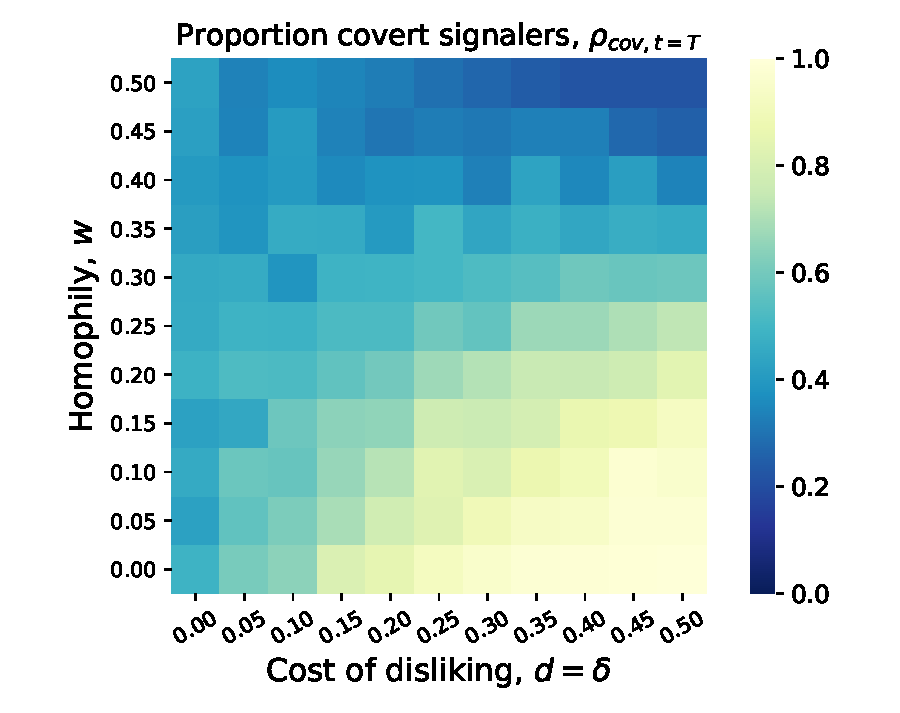
\includegraphics[width=\textwidth]{Figures/basic_disliking_signaling.pdf}
    \caption{Density of covert signalers.}
  \end{subfigure}
  \begin{subfigure}{0.49\textwidth}
    \centering
    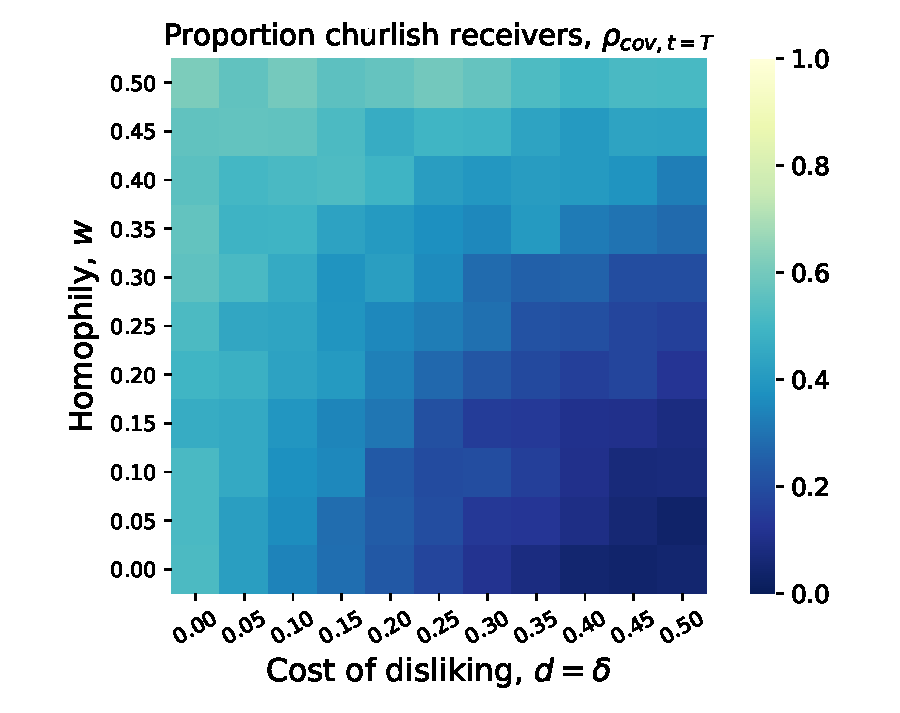
\includegraphics[width=\textwidth]{Figures/basic_disliking_receiving.pdf}
    \caption{Density of churlish receivers.}
  \end{subfigure}
  
  \caption{Density of covert signalers and churlish receivers at $t=500$, 
    the final timestep.}
  \label{fig:dislikingHomophilyHeatmap}
\end{figure}

\subsubsection{...as a function of covert signaling efficiency}

\begin{figure}[H]
  \centering
  \begin{subfigure}{0.49\textwidth}
    \centering
    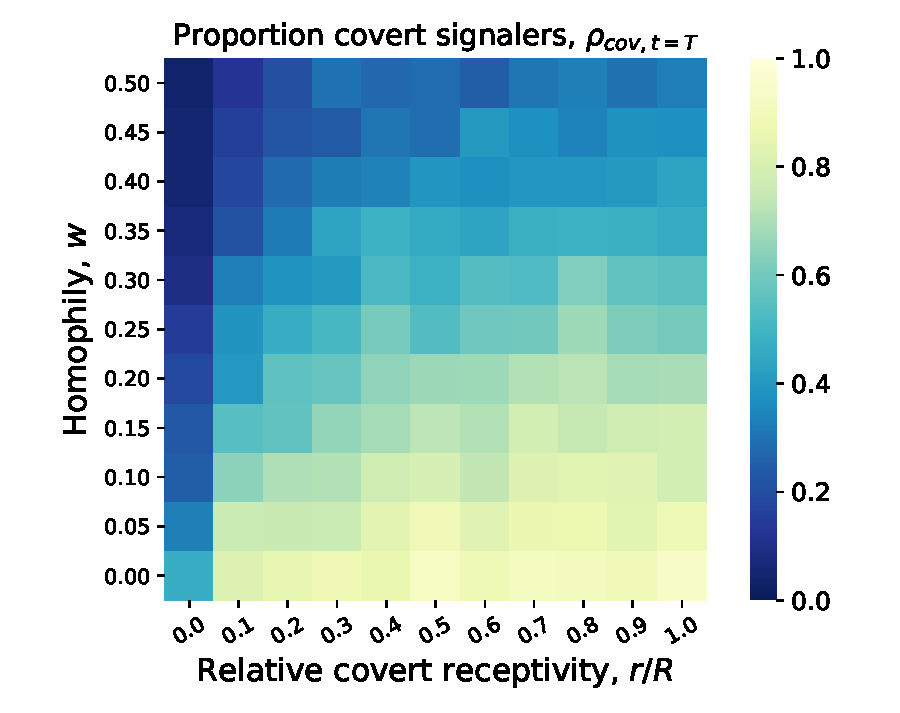
\includegraphics[width=\textwidth]{Figures/basic_receptivity_signaling.pdf}
    \caption{Density of covert signalers.}
  \end{subfigure}
  \begin{subfigure}{0.49\textwidth}
    \centering
    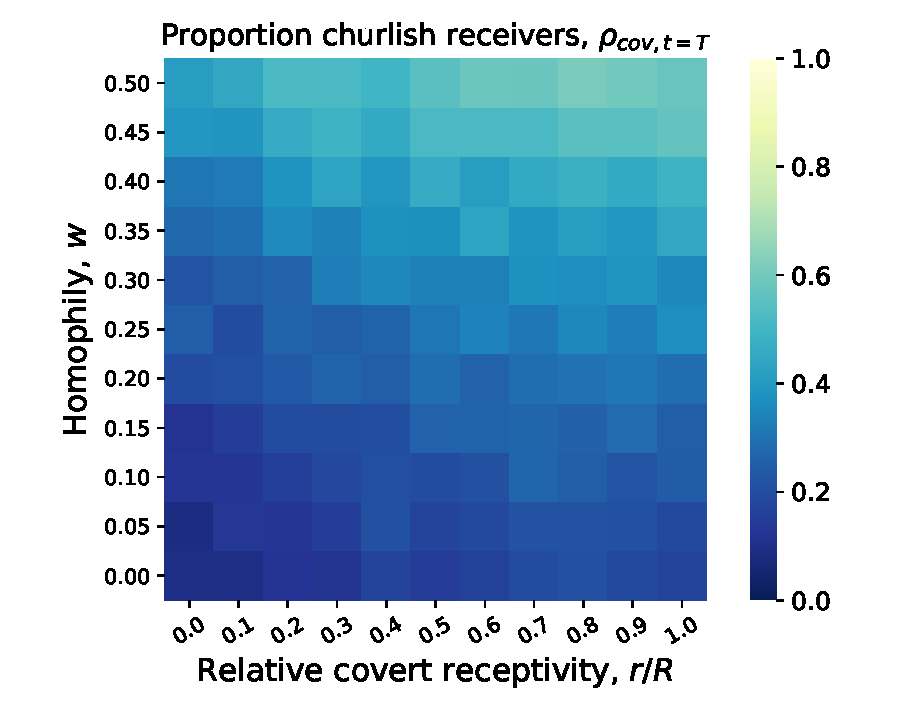
\includegraphics[width=\textwidth]{Figures/basic_receptivity_receiving.pdf}
    \caption{Density of churlish receivers.}
  \end{subfigure}
  
  \caption{Density of covert signalers and churlish receivers at $t=200$, 
    final timestep recorded in this preliminary experiment. Receptivity of
    overt signals is $R=0.5$.}
  \label{fig:receptivityHomophilyHeatmap}
\end{figure}

\subsubsection{Co-evolution of covert signaling and generous receiving}

Theoretically, conditions favorable for covert
signalers should also be favorable for generous receivers (TRUE??). Furthermore, 
an increase in covert signalers increases the pressure towards generous receiving.
With many covert signalers it is likely an agent will get no signal on a 
turn because they were receiving a signal from a covert signaler. Disliking
incurs a penalty, so it is better to remain neutral.

\begin{figure}[H]
  \centering
  \begin{subfigure}{0.49\textwidth}
    \centering
    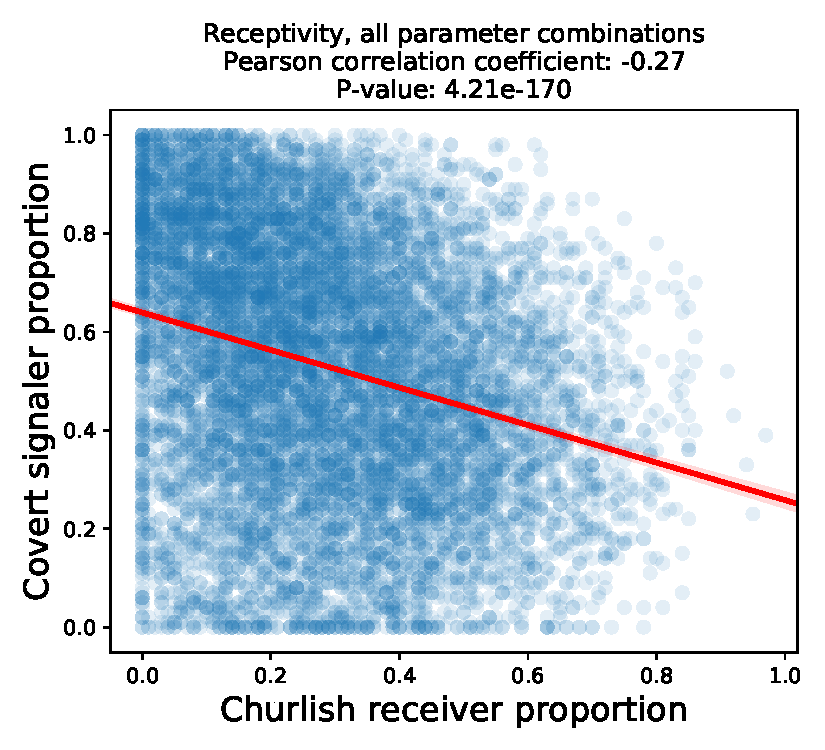
\includegraphics[width=\textwidth]{Figures/receptivity_allcombos_reg.pdf}
    \caption{}
    \label{fig:}
  \end{subfigure}
  \begin{subfigure}{0.49\textwidth}
    \centering
    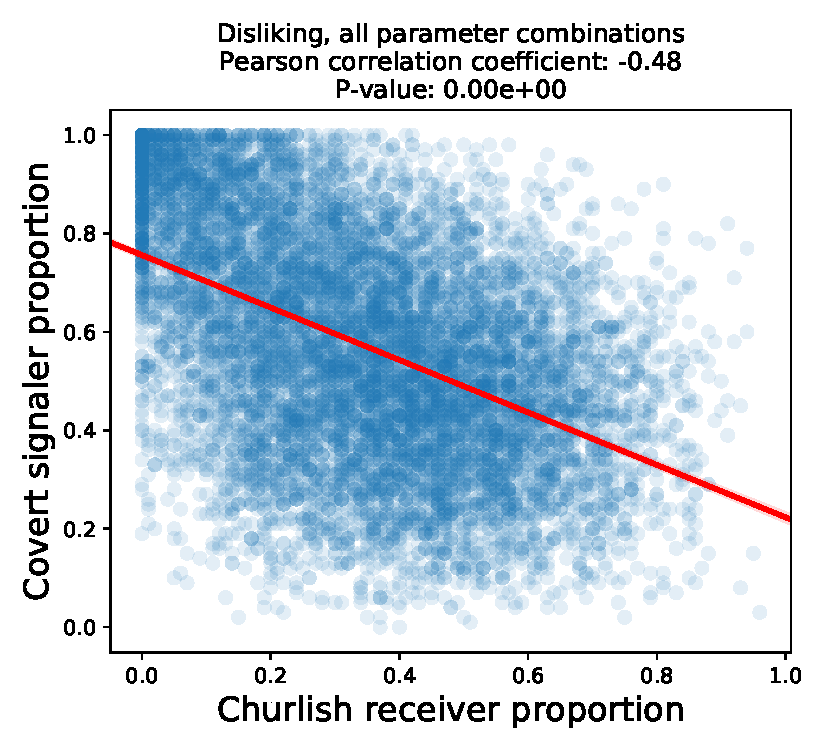
\includegraphics[width=\textwidth]{Figures/disliking_allcombos_reg.pdf}
    \caption{}
    \label{fig:}
  \end{subfigure}
  \caption{Correlation between proportion of covert signalers and proportion of
    churlish receivers for all tested parameter combinations in both 
    receptivity (a) and disliking (b) experiments. (NEED TO CHECK HOW I'M AVERAGING
    HERE AND POSSIBLY AGGREGATE FURTHER AS A SMOOTHING FILTER. ALSO NEED TO
    )}
  \label{fig:regressions}
\end{figure}


\subsection{Minority-majority dynamics}

Here we analyze the evolution of covert signaling in populations where there
are minority and majority sub-populations, as specified by agents' trait
vectors, $\tau_i$. In these experiments, the first $M$ of each agent's $K$ traits
are set to 1 or -1: fraction $\rho^{minor}$ of the
population is in the minority, and have the first $M$ of their traits set to
1, and the rest of the population is the majority, with the first $M$ of their
traits set to -1. 

We primarily vary the minority prevalence, $\rho^{minor}$, and set $M=1$ and
$K=3$, except for one heatmap in 
Figure~\ref{fig:covert-signaling-minority-heatmap}. 

\subsubsection{Covert minority signaling over minority prevalence}

\begin{figure}[H]
  \centering
  \begin{subfigure}{0.31\textwidth}
    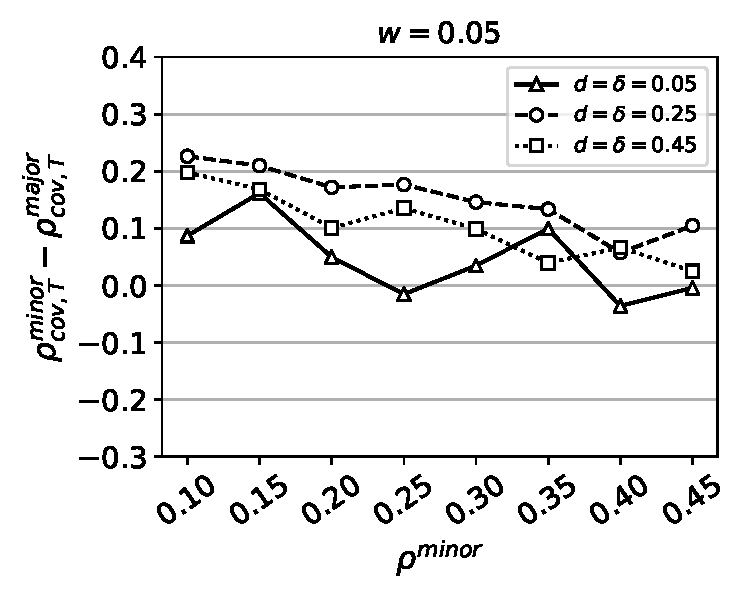
\includegraphics[width=\textwidth]{Figures/minority-homophily=0p05.pdf}
    \caption{}
  \end{subfigure}
  \begin{subfigure}{0.31\textwidth}
    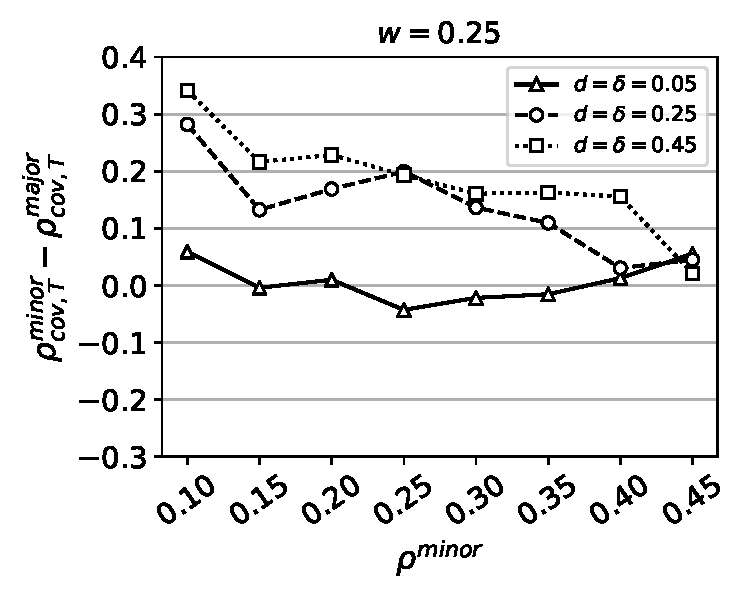
\includegraphics[width=\textwidth]{Figures/minority-homophily=0p25.pdf}
    \caption{}
  \end{subfigure}
  \begin{subfigure}{0.31\textwidth}
    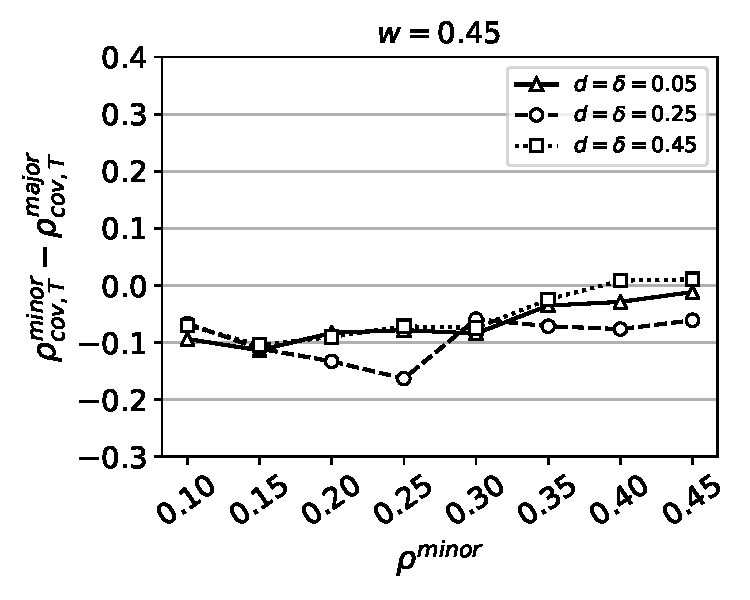
\includegraphics[width=\textwidth]{Figures/minority-homophily=0p45.pdf}
    \caption{}
  \end{subfigure}
  \caption{}
\end{figure}


\subsubsection{Minority covert signaling over homophily and disliking}

\begin{figure}[H]
  \centering
  \begin{subfigure}{0.48\textwidth}
    \centering
    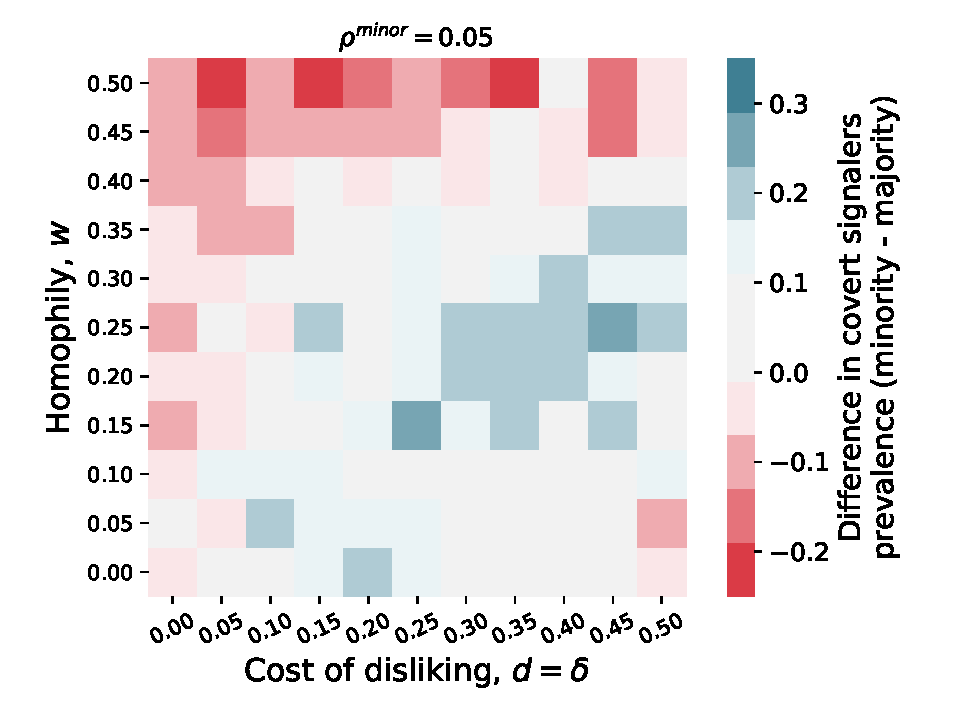
\includegraphics[width=\textwidth]{Figures/covert_signalers_diff_0p05.pdf}
    % \caption{Prevalence of minority covert receivers; $\rho^{minor} = 0.10$.}
  \end{subfigure}
  \hfill
  \begin{subfigure}{0.48\textwidth}
    \centering
    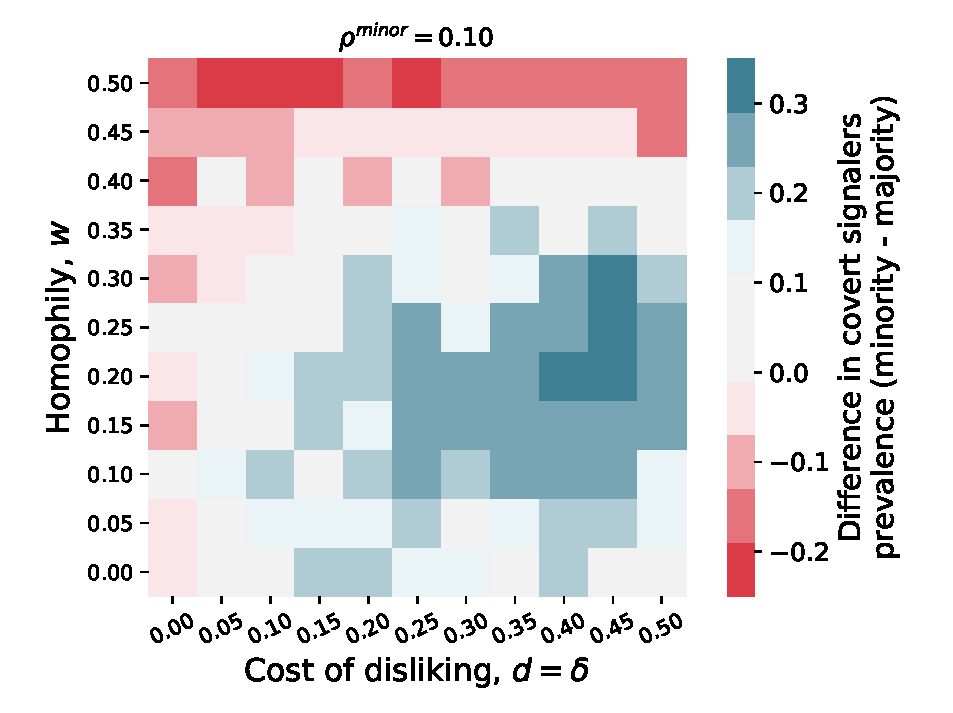
\includegraphics[width=\textwidth]{Figures/covert_signalers_diff_0p10.pdf}
    % \caption{Prevalence of minority covert receivers; $\rho^{minor} = 0.25$.}
  \end{subfigure} \\[.25in]
  \begin{subfigure}{0.48\textwidth}
    \centering
    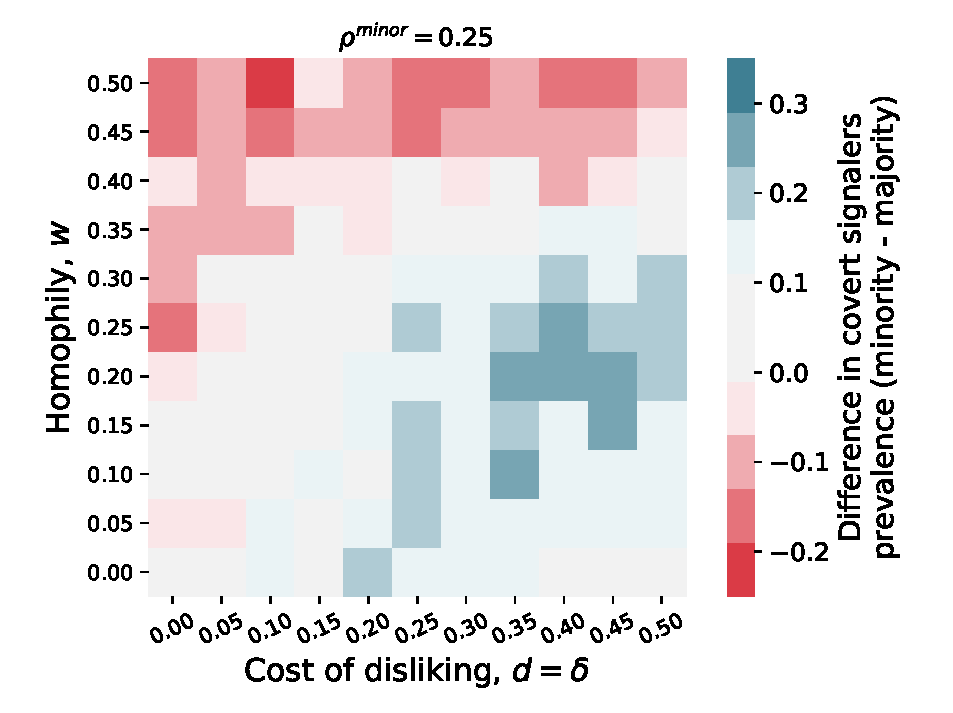
\includegraphics[width=\textwidth]{Figures/covert_signalers_diff_0p25.pdf}
    % \caption{Prevalence of minority churilsh receivers; $\rho^{minor} = 0.10$.}
  \end{subfigure}
  \hfill
  \begin{subfigure}{0.48\textwidth}
    \centering
    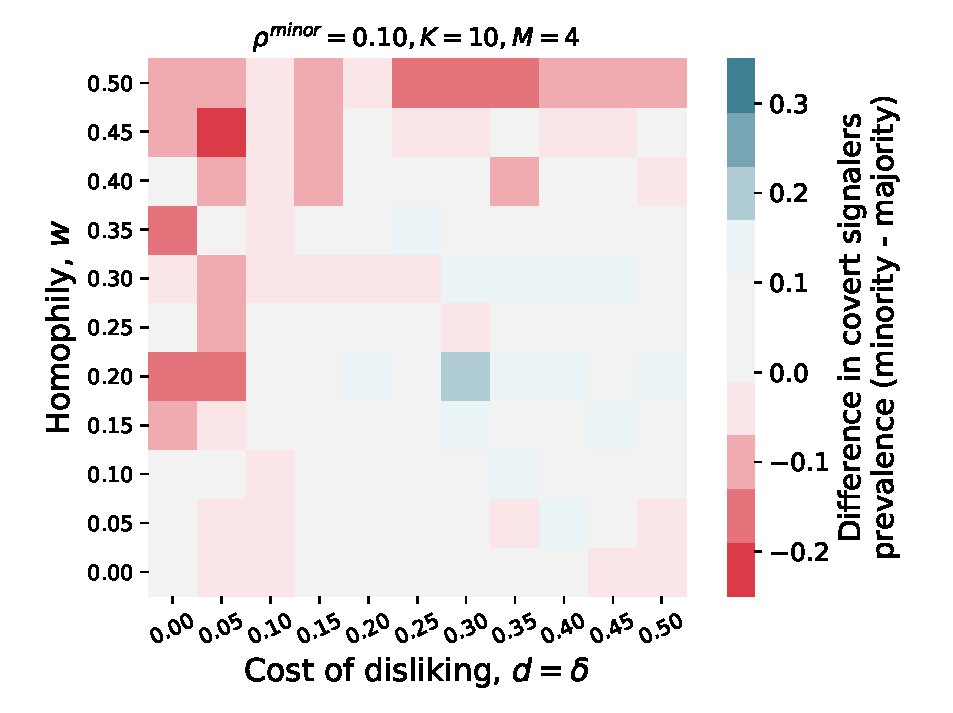
\includegraphics[width=\textwidth]{Figures/covert_signalers_diff_0p10_K=10_M=4.pdf}
    \caption{(NEED TO UPDATE WITH K=9 AND M=4. Ran these, just need to pull from
    MERCED and analyze.)}
  \end{subfigure}
  \caption{Difference in covert signaling prevalence between minority and
  majority populations for different parameters settings.}
  \label{fig:covert-signaling-minority-heatmap}
\end{figure}


\subsubsection{Minority churlish receiving over homophily and disliking}

\begin{figure}[H]
  \centering
  \begin{subfigure}{0.48\textwidth}
    \centering
    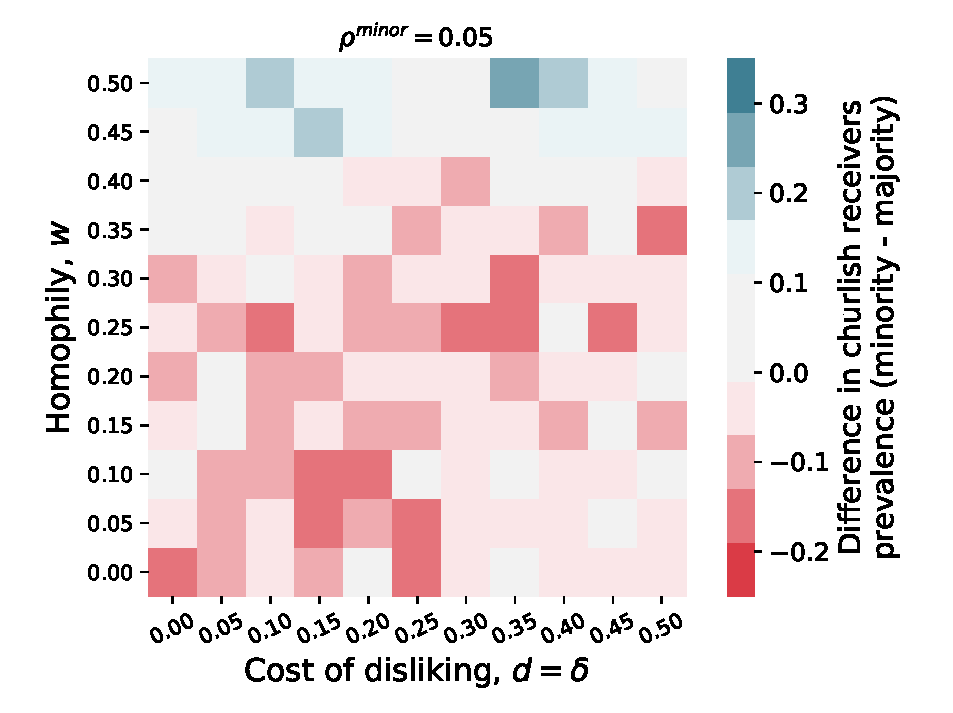
\includegraphics[width=\textwidth]{Figures/churlish_receivers_diff_0p05.pdf}
    % \caption{Prevalence of minority covert receivers; $\rho^{minor} = 0.10$.}
  \end{subfigure}
  \hfill
  \begin{subfigure}{0.48\textwidth}
    \centering
    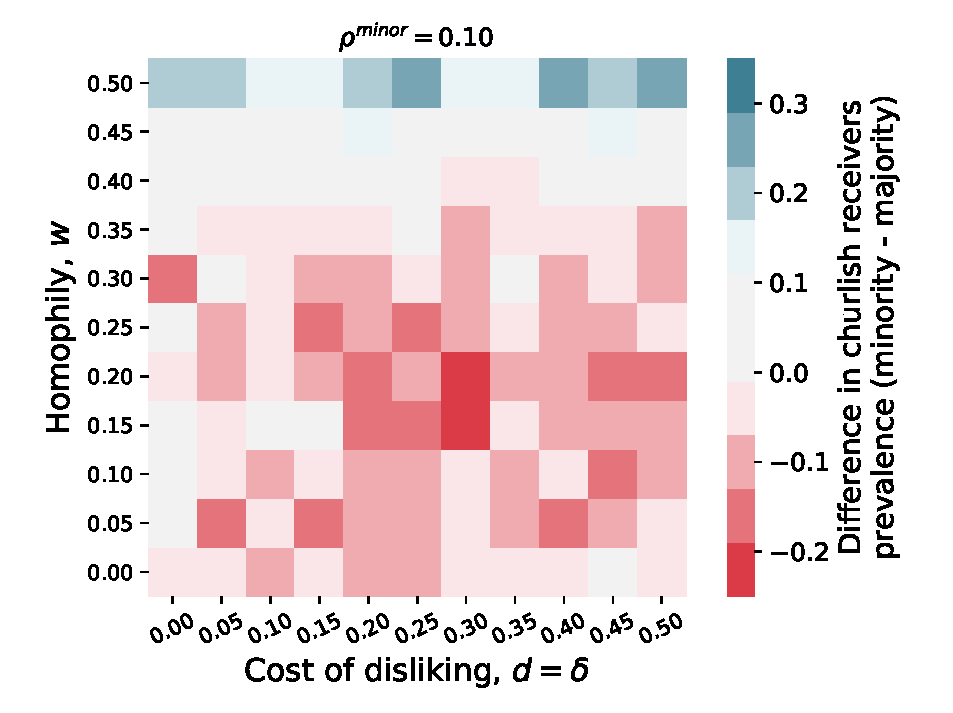
\includegraphics[width=\textwidth]{Figures/churlish_receivers_diff_0p10.pdf}
    % \caption{Prevalence of minority covert receivers; $\rho^{minor} = 0.25$.}
  \end{subfigure} \\[.25in]
  \begin{subfigure}{0.48\textwidth}
    \centering
    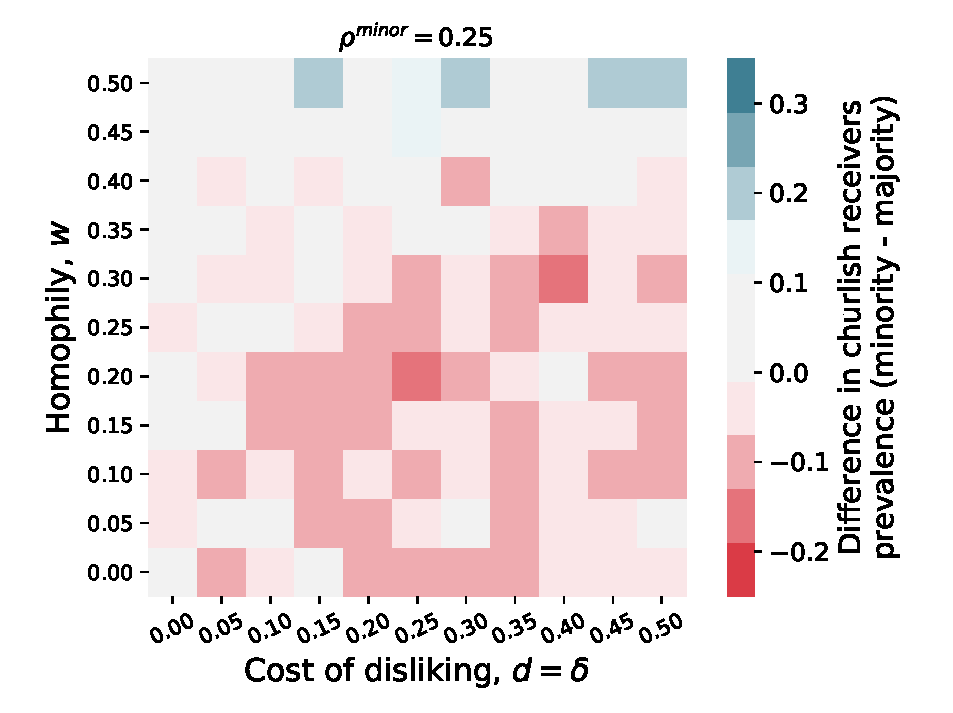
\includegraphics[width=\textwidth]{Figures/churlish_receivers_diff_0p25.pdf}
    % \caption{Prevalence of minority churilsh receivers; $\rho^{minor} = 0.10$.}
  \end{subfigure}
  \hfill
  \begin{subfigure}{0.48\textwidth}
    \centering
    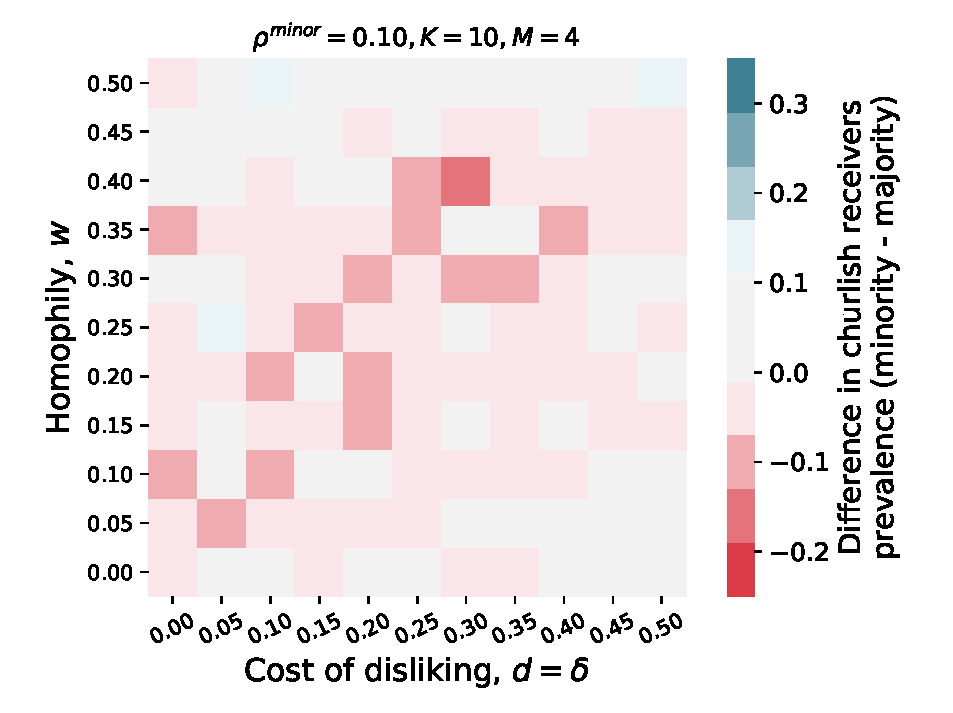
\includegraphics[width=\textwidth]{Figures/churlish_receivers_diff_0p10_K=10_M=4.pdf}
    % \caption{Prevalence of minority churilsh receivers; $\rho^{minor} = 0.25$.}
  \end{subfigure}
  \caption{Difference in churlish receiving prevalence between minority and majority
  populations for different parameter settings.}
\end{figure}

\subsection{Covert signaling invasion}

In this experiment we begin with initial proportions, $\rho$ of one of the strategies
at 0.05 and consider this the ``invading'' strategy. $\rho_{cov,0}$ represents
the initial covert proportion, $\rho_{ov,0}$ the initial overt proportion,
$\rho_{ch,0}$ the initial churlish proportion, and $\rho_{gen,0}$ the 
initial generous proportion. We measure how often
a non-zero proportion of agents with the invading strategy manage to 
establish a permanent population, which we call invasion success. We calculated
invasion success for a number of experimental parameter settings, covarying
over disliking penalty ($d=\delta$) and homophily ($w$) in the first case,
and over relative covert receptivity ($r/R$) and homophily ($w$) 
in the second case (Figures~\ref{fig:cov-ov-invade} and~\ref{fig:ch-gen-invade}).

\begin{figure}[H]
  \centering
    \begin{subfigure}{0.49\textwidth}
      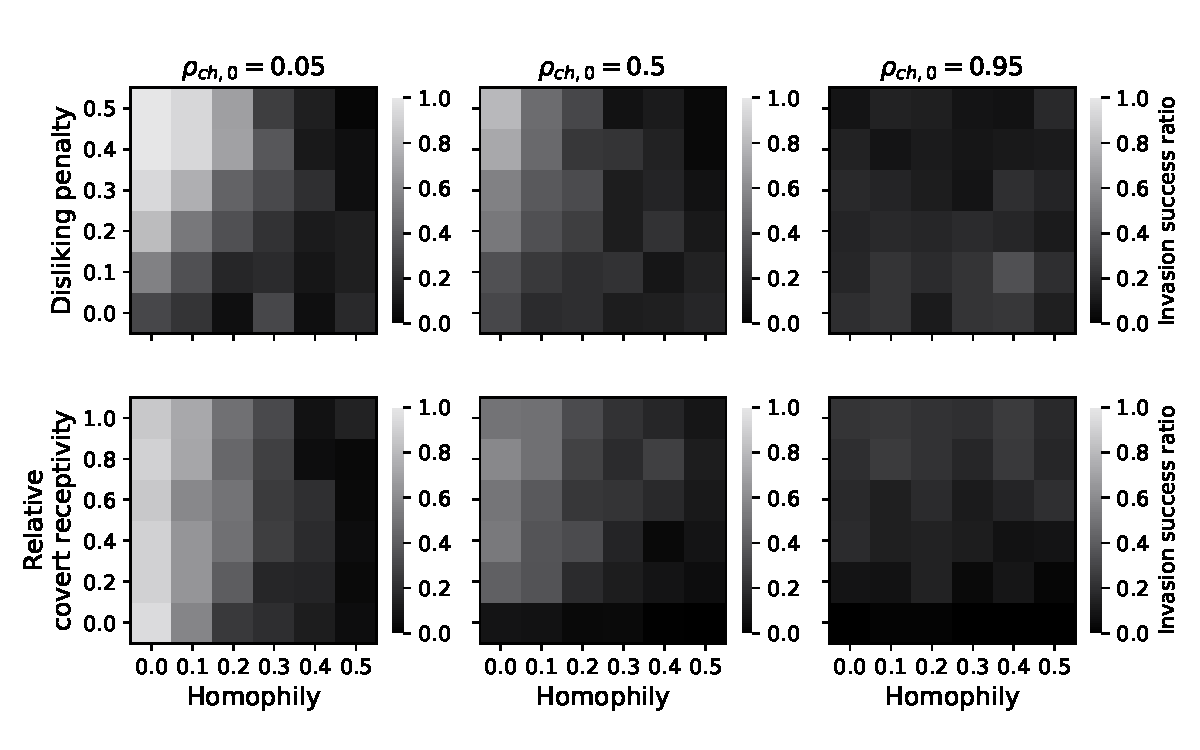
\includegraphics[width=\textwidth]{Figures/covert_invades.pdf}
      \caption{Covert invades, $\rho_{cov,0}=0.05$}
    \end{subfigure}
    \begin{subfigure}{0.49\textwidth}
      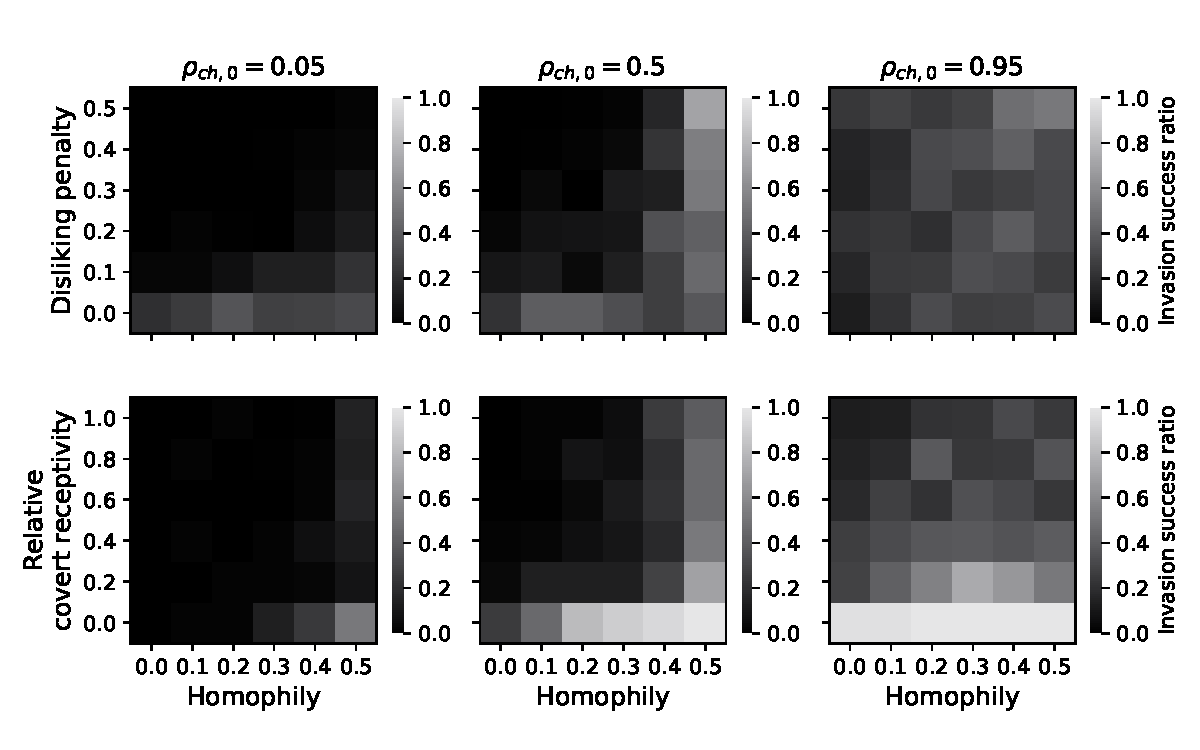
\includegraphics[width=\textwidth]{Figures/overt_invades.pdf}
      \caption{Overt invades, $\rho_{cov,0}=0.95$}
    \end{subfigure}
  \caption{Covert and overt sending strategy invasion success rates. 
    Lower homophily is more favorable for successful covert signaling invasion.
    This is due to lower homophily meaning agents cannot assort well into
    similar pairs prior to interaction.
    Similarly, greater homophily is more favorable for successful overt
    signaling invasion, where agents can better assort if they know each other's
    true traits. Unexpectedly, as covert receptivity increases, overt signaling
    is is more successful at invading and covert signaling is less successful
    at invading when the initial churlishness is high. When initial
    churlishness is small to moderate, the pattern is reversed.
  }
  \label{fig:cov-ov-invade}
\end{figure}

\begin{figure}[H]
  \centering
    \begin{subfigure}{0.49\textwidth}
      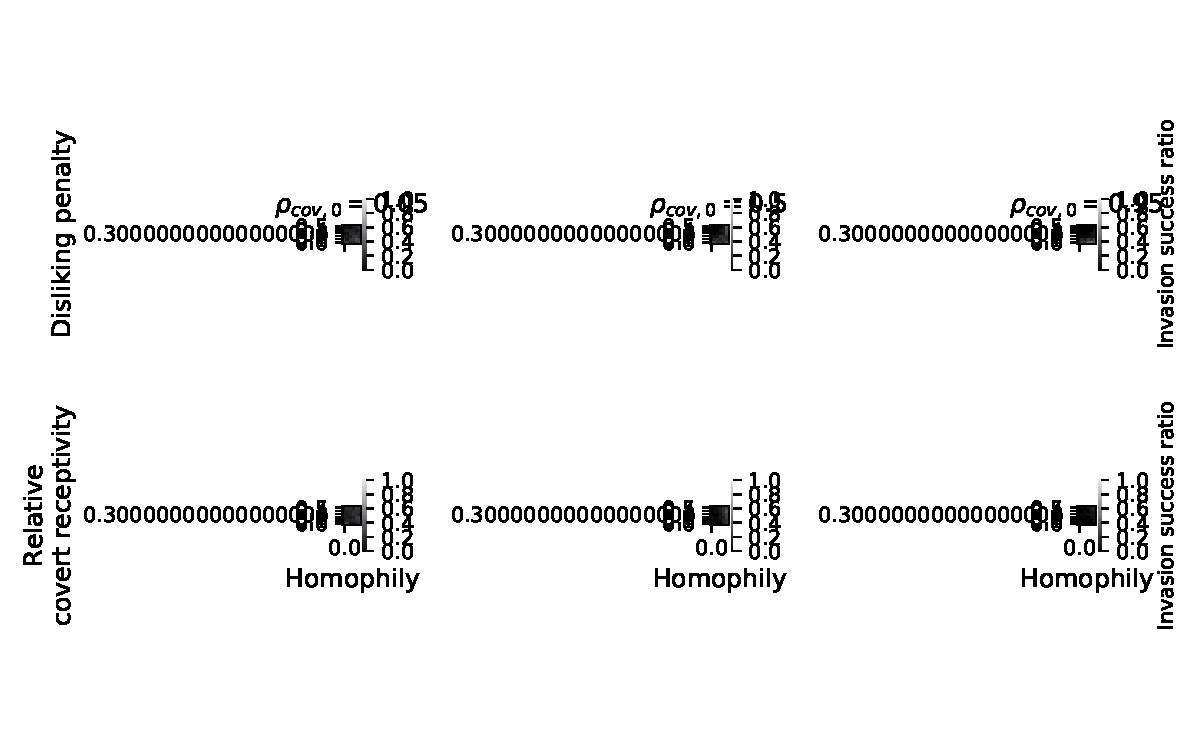
\includegraphics[width=\textwidth]{Figures/churlish_invades.pdf}
      \caption{Churlish invades, $\rho_{ch,0}=0.05$}
    \end{subfigure}
    \begin{subfigure}{0.49\textwidth}
      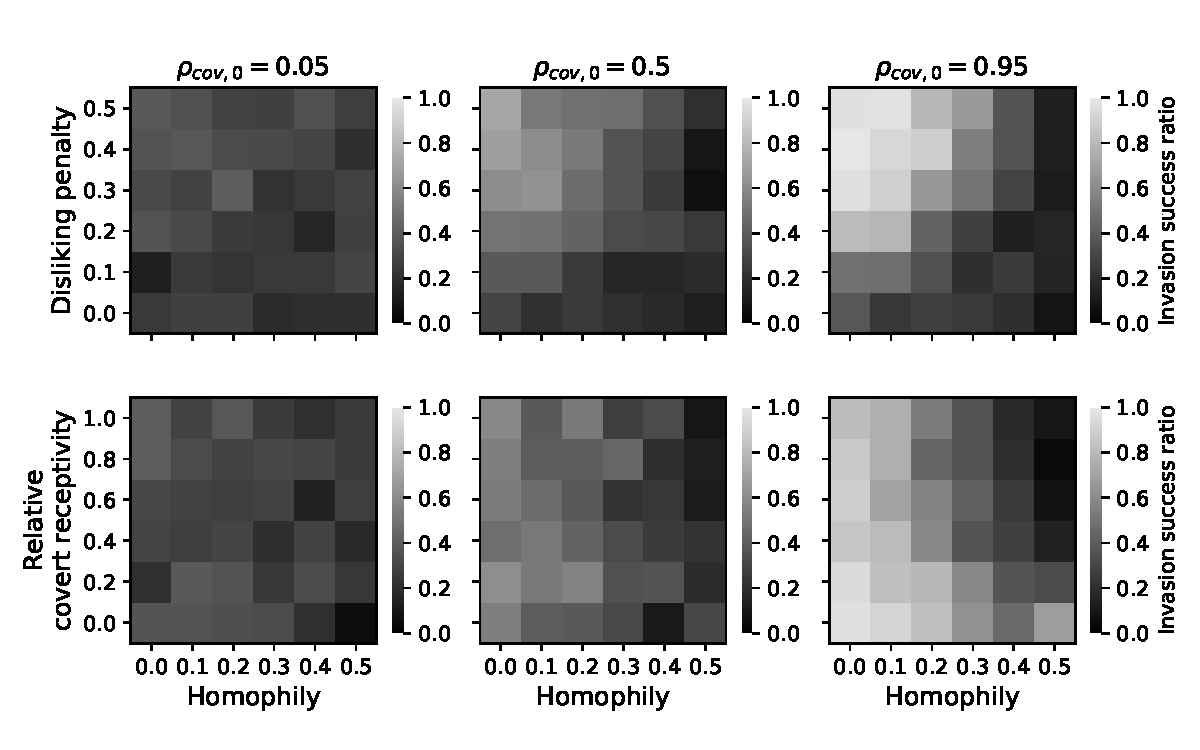
\includegraphics[width=\textwidth]{Figures/generous_invades.pdf}
      \caption{Generous invades, $\rho_{ch,0}=0.95$}
    \end{subfigure}
  \caption{Churlish and generous receiving strategy invasion success rates.
    For low to moderate rates of initial covert signaling there is not much
    of a pattern to invasion success. High values of homophily do seem to lead
    to more successful churlish invasion for moderate values of initial
    covert signalers. For large initial proportions of covert
    signalers, lower homophily favors generous invasion, which is more pronounced
    for larger disliking penalties.
  }
  \label{fig:ch-gen-invade}
\end{figure}

\subsubsection{Non-signaling as an adaptive strategy}

One of the most striking patterns in the invasion results is the evolution
of a third de facto strategy of non-signaling. This strategy emerges when
we consider both the invasion dynamics of either the covert or overt 
signaling strategy. When simulating the invasion of covert signaling
($\rho_{cov,0}=0.05$), the non-signaling strategy emerges when the covert
signaling efficiency, $r$, is 0, but covert signaling still successfully
invades as the chosen agent strategy. When $r=0$, no agents receive
covert signals, making this more accurately a \emph{non-signaling} strategy.  
For covert signaling invasion, this only happens when the initial churlishness
is low ($\rho_{ch,0}=0.05$) and homophily is also low ($w \lessapprox 0.2$). 
Non-signaling wins out evolutionarily 
in some cases when considering of invading overt signalers when overt signalers
fail to invade but $r=0$, again meaning agents in this society prefer not
to signal at all. This occurs some of the time for all tested homophily
values and low initial churlishness ($\rho_{ch,0}=0.05$) (Figure~\ref{fig:cov-ov-invade}b, bottom left plot).  
Overt signaling continues to fail to evolve at least some of the time
for $r=0$ for moderate initial churlishness ($\rho_{ch,0}=0.5$) up up to perfect 
assortment homophily, $w=0.5$.

% \bibliographystyle{apacite}

% \setlength{\bibleftmargin}{.125in}
% \setlength{\bibindent}{-\bibleftmargin}

% \bibliography{/Users/mt/workspace/papers/library.bib}

\appendix

\section{Additional analyses}

\subsection{Temporal dynamics}

\subsection{Correlations between churlish receiving and covert signaling}

\subsection{$d \neq \delta$}

Vary $\delta$ from 0 to $2d$.

\subsection{Minority dynamics} 

\subsubsection{More traits ($K=9$ and $M=4$) and different similarity threshold}

\subsubsection{Varying minority group size}

\subsection{Invasion of other strategies}


\section{Model implementation}

In order to aid evaluation of our model code, we provide notes below on 
our model implementation. The code is freely available on GitHub at
\url{https://github.com/mt-digital/identity-signaling}.

\end{document}
